\documentclass[12pt]{article}

\usepackage[spanish]{babel}
\usepackage{amsfonts}
\usepackage[utf8]{inputenx}
\usepackage{algorithm2e}
\usepackage{listings}
\usepackage{pdfpages}

\usepackage{color}
\definecolor{deepblue}{RGB}{0,0,153}
\definecolor{deepred}{RGB}{153,0,0}
\definecolor{deepgreen}{RGB}{51,102,0}
\definecolor{deepyellow}{RGB}{204,204,0}

\lstset{ %
			language=Python,
			basicstyle=\footnotesize,
			numbers=left,
			stepnumber=1,
			numbersep=4pt,
			tabsize=2,
			otherkeywords={self}, 
			keywordstyle=\color{deepred},
			stringstyle=\color{deepgreen},
			commentstyle=\color{deepblue},
}
\usepackage{hyperref}
\hypersetup{
    colorlinks=true,
    citecolor=black,
    filecolor=black,
    linkcolor=black,
    urlcolor=black,
    linktoc=all
}


\title{Distancia de Edición}
\author{
        Alejandro Pernin \\
                \and
        Lautaro Medrano\\
}
\date{\today}



\begin{document}
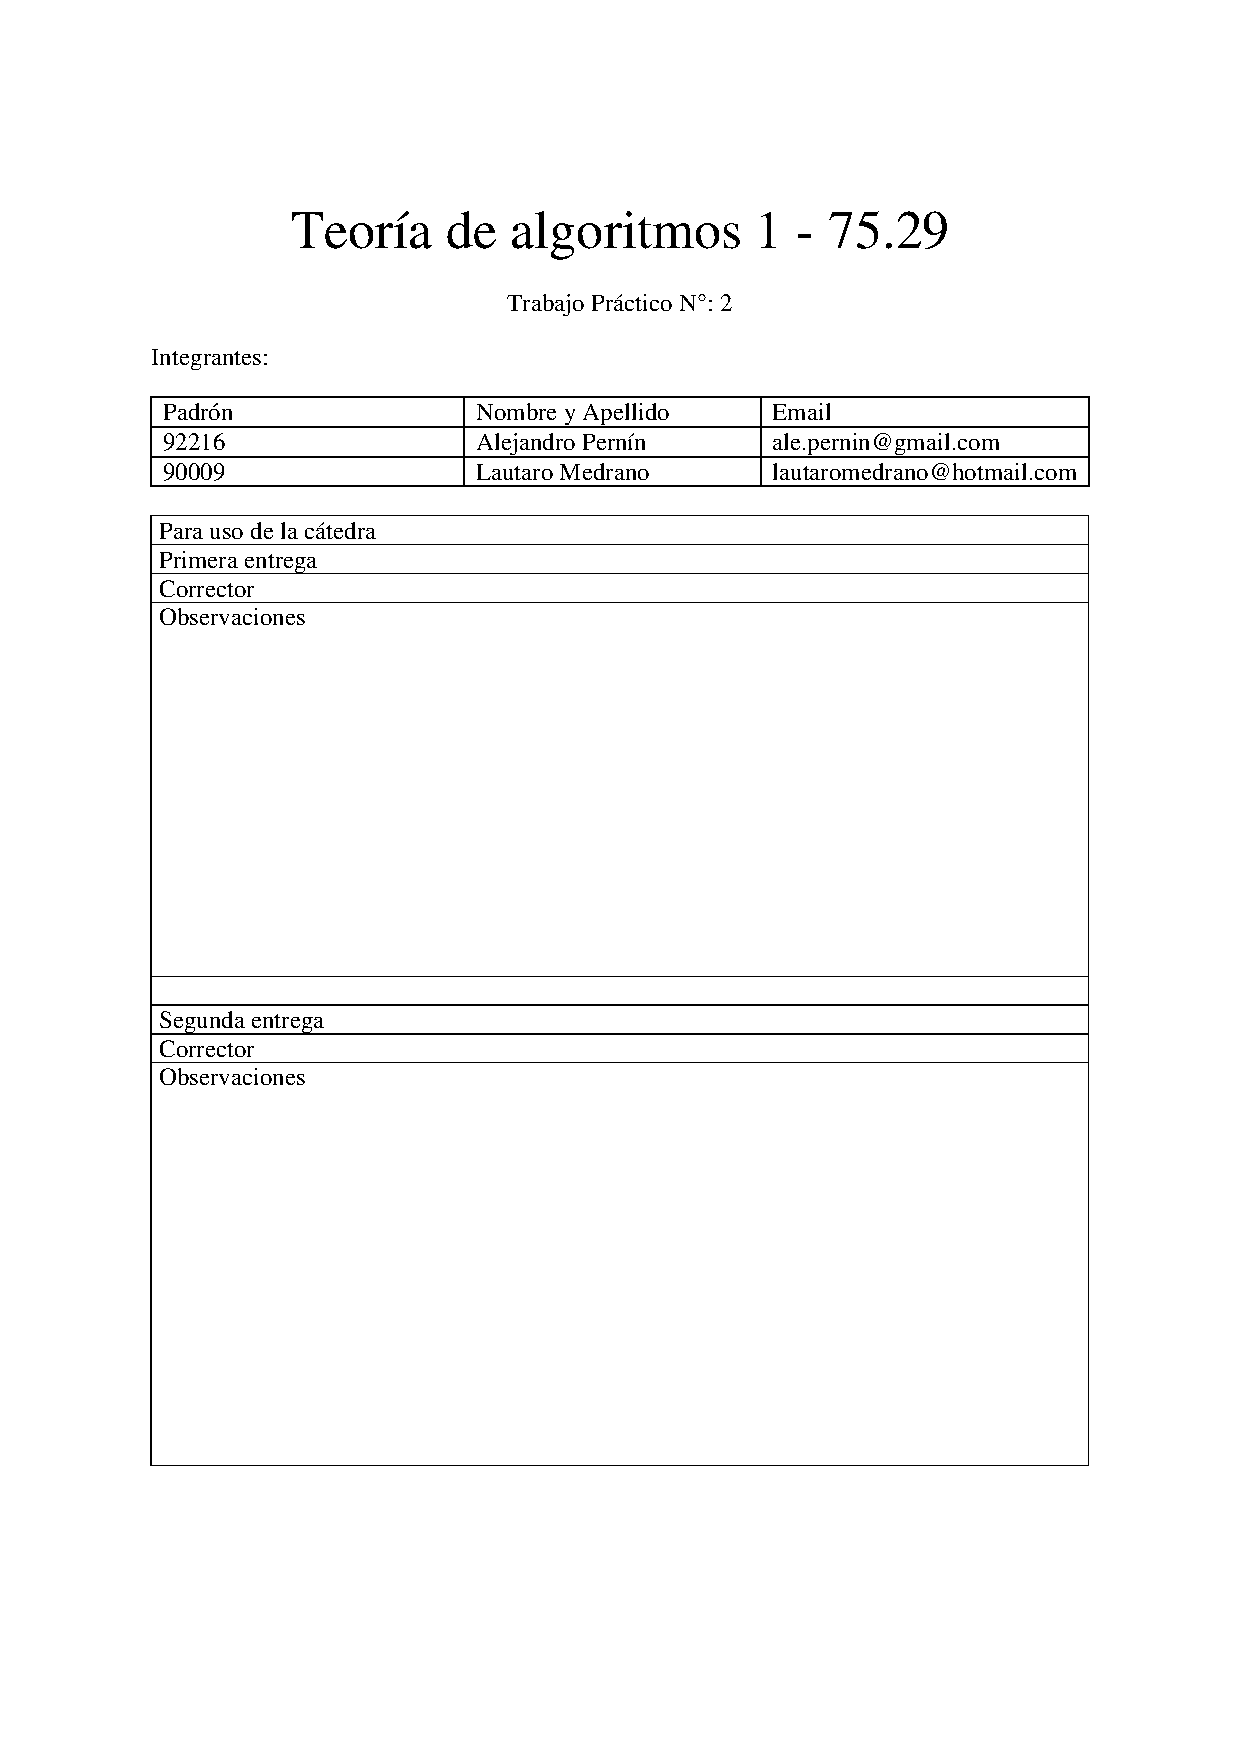
\includepdf{caratula.pdf}

\maketitle

\newpage
\tableofcontents

\newpage

\section{Enunciado}
\textbf{\underline{Distancia de edición}}
Para convertir una cadena de caracteres x [1..m ] en otra cadena y [1..n ] , se pueden
realizar distintas operaciones. La meta consiste, en dadas las cadenas x e y ,
encontrar una serie de transformaciones para cambiar x en y , para lo cual debemos
emplear un vector z (cuyo tamaño asumimos que es suficiente para almacenar todos los
caracteres necesarios) en el que almacenaremos los resultados parciales. Al inicio z
está vacío y al final se cumple que z [ j ]= y [ j] para j=1,2 , ... , n . Se deben examinar
todos los caracteres de x , para lo cual se mantienen los índices i en x y j en z .
En un principio i= j=1 y al final i=m+ 1 . En cada paso se aplica alguna de las
siguientes seis operaciones (transformaciones):
\\\\
\textbf{Copiar:}copia un carácter de x a z . Esto es: z [ j ]= x [i ] e incrementa los índices i
yj
\\\\
\textbf{Reemplazar:}reemplaza un carácter de x por otro carácter c . Esto es: z [ j ]=c e
incrementa los índices i y j
\\\\
\textbf{Borrar:}borra un carácter de x incrementando i y sin mover j
\\\\
\textbf{Insertar:} inserta un carácter c en z . Esto es: z [ j ]=c e incrementa j sin mover i
\\\\
\textbf{Intercambiar:} intercambia los próximos dos caracteres copiándolos de x a z pero en
orden inverso. Esto es: z [ j ]= x [i+ 1] y z [ j +1]= x [i ] e incrementa los índices de la
siguiente manera: i=i+2 y j= j+2
\\\\
\textbf{Terminar:} elimina los caracteres restantes de x haciendo i=m+ 1 . Esta operación
descarta todos los caracteres de x que todavía no se analizaron. Es la última operación
se aplica si hace falta.

\newpage
\subsection{Distancia de edición}
Dadas dos cadenas x [1..m] e y [1..n ] y el costo de cada una de las operaciones
. Escribir un programa (programación dinámica) que calcule la distancia de edición
siendo esta la secuencia de menor costo que permita transformar x en y .
Analizar la complejidad en tiempo y espacio de la solución implementada.
El programa debe tomar como parámetros las dos cadenas y el nombre de un
archivo con el costo de las operaciones. El formato de cada línea de este archivo
es el siguiente:

\verb# <operacion>:<costo>#

Ejemplo de invocación: \emph{tdatp2 algoritmo altruista costos.txt}

La salida debe ser por pantalla y debe mostrar una línea por cada operación,
indicando los caracteres que se insertan o reemplazan. Una línea en blanco y el costo total de
la secuencia.

\subsection{Alineación secuencias ADN}
El problema de la distancia de edición, tal como está planteado en este TP generaliza el
problema de alinear dos secuencias de ADN. Existen varios métodos para medir la
similitud entre dos secuencias de ADN alineándolas. Uno de esos métodos consiste en
insertar espacios en posiciones arbitrarias en ambas secuencias (incluyendo al final) tal
que las secuencias resultantes tengan la misma longitud pero que no tengan espacios en
la misma posición. Entonces se le asigna un puntaje a cada posición de la siguiente
manera:

\begin{itemize}
	\item +1 si $x'[j]=y'[j]$ y ninguno es un espacio
	\item -1 si $x'[j]\neq y'[j]$ y ninguno es un espacio
	\item -1 si $x'[j]$ o $y'[j]$ es un espacio
\end{itemize}

El puntaje total de la alineación es la suma de los puntaje de cada posición. Por ejemplo
dadas las secuencias x=GATCGGCAT e y=CAATGTGAATC, una alineación posible
es:
\[
\begin{array}{ccccccccccccc}
  &G &\space &A &T &C &G &\space &G &C &A &T &\space  \\
  &C &A &A &T &\space &G &T &G &A &A &T &C	\\
  &-1 &-2 &+1 &+1 &-2 &+1 &-2 &+1 &-1 &+1 &+1 &-2
\end{array}
\]
Tal que el puntaje total de la alineación es $6*1-2*1-4*2=-4$
Explicar que como utilizar el programa de distancia de edición del punto 1
utilizando un subconjunto de las operaciones copiar, reemplazar, borrar, insertar,
intercambiar y terminar para resolver el problema de la alineación de secuencias de
ADN con el método dado.

\newpage
\section{Resolución}
\subsection{Distancia de edición}
Para la resolución de los problemas planteados se tuvieron en cuenta
algunas hipótesis:

\begin{itemize}
	\item El costo individual de copiar y reemplazar, son menores que los costos de las
combinaciones de borrar e insertar.
	\item Conozco soluciones parciales anteriores del problema.
	\item El problema es case sensitive, por lo cual mayúsculas y minúsculas serán
diferenciadas.
	\item Las operaciones estan sujetas a prohibición.
\end{itemize}

El problema se atacó desde un punto de vista dinámico utilizando el enfoque de
memorización, es decir que se van guardando en memoria soluciones previas a un problema
menor, cuya solución considero es óptima.
Para ello se utilizó un diccionario que irá alojando las soluciones previas para tenerlas
disponibles para ensamblar soluciones futuras. El concepto de solución es:
\begin{itemize}
	\item $S_{n}=S_{n-1}+s(n)$
\end{itemize}

Es decir que la solución hasta un carácter se compone de la solución hasta el carácter anterior
más una solución para ese único carácter.

Para la composición de la solución se hace uso de la hipótesis de que la
copia es la mejor operacion a realizar (menor costo), para poder realizar
una toma de decisiones se utiliza como recursos el resultado obtenido de
una implementación de LCS\footnote{Longest Common Sequence - Secuencia Común más Larga}
y un análisis de la diferencia de tamaños entre la base y el objetivo.

Algunas de las consideraciones que se toman en cuenta son:
\begin{itemize}
	\item Si $base(pos)\in LCS \rightarrow$ es un caracter que se puede 
	copiar, si se puede copiar esa misma instancia u otra con sus respectivos
	impactos.
	\item Si $|base| <= |objetivo| \rightarrow$ borrar un caracter implica 
	a futuro una inserción.
	\item Si $|base| >= |objetivo| \rightarrow$ una inserción puede a futuro
	implicar un borrar o terminar.
\end{itemize}

Teniendo en cuenta estas consideraciones se hace un análisis de costos y 
de que operación es la óptima a efectuar.
\\

\begin{algorithm}[H]
	\SetAlgoLined
	
	\KwData{n}
	\KwResult{lista\_solucion }
	
	\If {$post == 0$}{
			return $s(n)$;
	}
	\If {$!Dict_{n-1}$}{
			$Dict_{n-1}=S_{n-1}$\;
	}
	\If {$!Dict_{n}$}{
			$Dict_{n-1}=Dict_{n-1}+s(n)$\;
	}
	$l\leftarrow Dict_{n}$\;
	return $l$;

\caption{Obtención $S_{n}$ con memorización}
\end{algorithm}

\subsection{Alineación secuencias ADN}
Para la resolución del problema de alinear secuencias de ADN se utiliza 
el mismo algoritmo utilizado para la distancia de edición, utilizando un
conjunto de operaciones adaptados a este problema. Para hallar que operaciones
y que respectivos costos se debieran utilizar se hizo un analisis del problema.
Veamos el ejemplo de alineación:

\[
\begin{array}{clcccc}
 & &1 &2 &3 &4 \\
  &base: &G &\space &A &C \\
  &objetivo: &C &A &A&\space \\
  &costo: &-1 &-2 &+1 &-2 
\end{array}
\]

\begin{itemize}
	\item 1) Representa un reemplazo con un costo de -1.
	\item 2) Representa una inserción con un costo de -2.
	\item 3) Representa un copiar con un costo de +1.
	\item 4) Representa un borrar con un costo de -2.
	\item No se realizan operaciones terminar o intercambiar.
\end{itemize}

El objetivo de la alineación es obtener aquella alineación cuyo puntaje
es máximo, pero siendo que el algoritmo a utilizar trabaja con mínimos,
lo que se debe realizar es invertir los costos (eg: Copiar:-1); asi mismo
el resultado que obtendremos también debemos invertirlo para que represente
el puntaje máximo.
Por ejemplo el archivo de costos a utilizar sería:
\begin{lstlisting}
reemplazar:1
insertar:2
borrar:2
copiar:-1
\end{lstlisting}

Utilizando este archivo para la resolución de las secuencias dadas como
ejemplo obtenemos:
\begin{lstlisting}
reemplazar g c
copiar a
insertar a
copiar t
reemplazar c g
reemplazar g t
copiar g
reemplazar c a
copiar a
copiar t
insertar c

El costo es: 3
\end{lstlisting}
Cuyo puntaje de alineacion es -3 y equivale a:
\[
\begin{array}{ccccccccccccc}
  &G &\space &A &T &C &G &G &C &A &T &\space  \\
  &C &A &A &T &G &T &G &A &A &T &C	\\
  &-1 &-2 &+1 &+1 &-1 &-1 &+1 &-1 &+1 &+1 &-2
\end{array}
\]

\newpage
\section{Análisis de orden}
A continuación se hará un análisis de los órdenes de los principales
módulos que se utilizan en la resolución del problema. Se omiten aquellos
que no revisten complejidad y/o relevancia, pero cuyo análisis igual se
encuentra en el código fuente\footnote{Ver \ref{sec:sourcecode}}.

\begin{itemize}
	\item LCS\footnote{Ver \ref{subsec:lcs}}: El algoritmo consta
	de tres segmentos, el costo total es la suma de los costos individuales.
	
	$O(|base|+1 * |obj|+1)+O(|base|*|obj|)+O(|base|*|obj|)$
	
	$O(|base|+1 * |obj|+1)=O(|base|*|obj|+|base|+|obj|+1)<O(3*|base|*|obj|)=O(|base|*|obj|)$
	\\Por propiedades de O, el orden total es:
	\\$O(|base|*|obj|)$
	
	\item solve()\footnote{\label{pie1}Ver \ref{subsec:tdatp2}}: Todas las operaciones realizadas son $O(1)$, hay un llamado
	recursivo, pero de profundidad 1; por lo que se puede asegurar que el 
	costo total de este módulo es $O(1)$
	
	\item solution(): Por cada elemento de la palabra objetivo, se analiza
	si existe o no solución en tiempo constante. $O(|obj|)$
	
	\item La solución total se compone de efectuar un llamado a LCS y a 
	solution(), siendo $O(|obj|)<O(|obj|*|base|)$ por propiedades de O
	la cota superior de todo el problema es $O(|base|*|obj|)$
	
	Si tomamos $N=max\{|base|,|obj|\}$ podemos decir que $O(|base|*|obj|)<O(N^{2})$
\end{itemize}

\newpage
\section{Ejecución y pruebas}
	Siendo que el lenguaje utilizado es Python, no es necesaria ninguna 
	compilación. El programa se puede ejecutar directamente mediante el 
	siguiente formato:
	
	\verb#  python tdatp2 <base> <objetivo> <archivo costos>#
	\\o bien: 
	
	\verb# ./tdatp2 <base> <objetivo> <archivo costos>#
	
	Asimismo se incluye un conjunto de datos de prueba y scripts para 
	ejecutar pruebas de manera sencilla, dichos scripts se encuentran 
	escritos en lenguaje bash para ser ejecutados en enturnos UNIX.
	
	Para la primera parte del enunciado, se dan 4 conjuntos de datos, 
	para realizar pruebas con los mismos se debe invocar al script $test.sh$ 
	de la siguiente manera:
	
	\verb# ./test.sh [1-4]#
	
	De similar modo para ejecutar la prueba del ejemplo de alineación de
	secuencias de ADN, se provee del archivo de datos mencionado con 
	anterioridad y un script de prueba $adntest.sh$ cuya invocación es directa:
	
	\verb# ./adntest.sh#
	
\newpage
\section{Conclusiones}
	Se diseñó e implementó un algoritmo para analizar las operaciones 
	necesarias para transformar una palabra en otra, considerando una
	serie de costos asociados.
	
	Se hace un análisis del entorno del problema, para analizar las 
	posibles implicancias de una operación y preveer costos a futuro
	que puede acarrear efectuar la misma.
	
	Se utilizaron estructuras que al a vez de permitir almacenar en 
	memoria soluciones parciales del problema, permitan tener un acceso
	a las mismas en un tiempo óptimo.
	
	Asimismo se analizó de que manera con sólo modificar los datos de 
	entrada y haciendo una conversión del resultado; se puede utilizar 
	el mismo algoritmo para solucionar un problema para el cual no fue
	diseñado originalmente.
	
	Se obtuvo un algoritmo que obtiene una solución en un tiempo polinomial $O(N^{2})$.

\newpage
\section{Modificaciones}
	La solución acá presente es el resultado de la modificación de una
	solución planteada con anterioridad, pero que no cumplia ciertos
	objetivos. A continuación se detallan algunas de las modificaciones:
	\begin{itemize}
		\item La solución anterior no era óptima, se analizaban las condiciones
		locales caracter a caracter, no teniendo en cuenta las futuras 
		implicancias de una operación. Por lo que aún siendo una operación
		óptima para la obtención del carácter deseado, esa operación a 
		futuro podría acarrear realizar operaciones que aumetasen el costo
		total.
		\item Con razón de proveer de información para la toma de decisiones
		necesarias descriptas en el item anterior, se añadió implementó
		el algoritmo de LCS.
		\item Se considera la posibilidad de prohibir operaciones.
		\item Se efectua un análisis más global del contexto del programa
		(diferencia de tamaños, operaciones previas, etc).
	\end{itemize}

\newpage
\section{Referencias}
	\begin{itemize}
		\item Wikipedia: Big O Notation - \url{http://en.wikipedia.org/wiki/Big_O_notation}
		\item Python Wiki: Time Complexity - \url{https://wiki.python.org/moin/TimeComplexity}
		\item `Introduction to Algorithms'- Cormen, Leiserson, Rivest, Stein -(ISBN:0-262-03293-7)
		\item `Algorithm Desing' - Kleinberg, Tardos - (ISBN: 0-321-29535-8)
	\end{itemize}
\newpage
\section{Codigos Fuente}\label{sec:sourcecode}
\subsection{LCS.py}\label{subsec:lcs}
\lstinputlisting{LCS.py}

\newpage
\subsection{tdatp2.py}\label{subsec:tdatp2}
\lstinputlisting{tdatp2.py}
\end{document}
